\documentclass[aspectratio=169,xcolor=table]{beamer}
\usepackage{tikz}
\usetikzlibrary{shapes,arrows,positioning,fit,calc,backgrounds}
\usepackage{listings}
% xcolor with table option loaded via documentclass
\usepackage{booktabs}

% Theme - Simple, no shadows
\usetheme{default}
\usecolortheme{default}
\setbeamertemplate{navigation symbols}{}
\setbeamertemplate{footline}[frame number]

% Reduce spacing to prevent content cutoff
\setbeamersize{text margin left=5mm,text margin right=5mm}
\setlength{\parskip}{0.3em}
\setlength{\itemsep}{0.2em}

% Colors
\definecolor{picolor}{RGB}{46,139,87}
\definecolor{awscolor}{RGB}{255,140,0}
\definecolor{browsercolor}{RGB}{70,130,180}

% Title
\title{Distributed AI-Powered Argument Analysis System}
\subtitle{Real-Time Emotion Classification and Multi-Source Fact-Checking}
\author{Ifesi Onubogu\\ Siyao Yu\\Xintong Li \\Anyongyong Zhao}
\institute{AIoT Project}
\date{\today}

\begin{document}

% ====================
% TITLE SLIDE
% ====================
\begin{frame}
\titlepage
\end{frame}

% ====================
% OUTLINE
% ====================
\begin{frame}{Outline}
\tableofcontents
\end{frame}

% ====================
% SECTION 1: OVERVIEW
% ====================
\section{Project Overview}

\begin{frame}{Problem Statement}
\begin{block}{Challenge}
In an era of increasing polarization and misinformation, how do we:
\begin{itemize}
    \item Analyze emotional dynamics in real-time conversations?
    \item Verify factual claims against authoritative sources?
    \item Present crowd-sourced predictions for subjective statements?
\end{itemize}
\end{block}

\vspace{0.5cm}

\begin{block}{Solution}
A distributed edge-cloud system that:
\begin{itemize}
    \item Captures and processes conversations on Raspberry Pi
    \item Analyzes emotions using fine-tuned transformers on AWS
    \item Fact-checks claims via RAG, Polymarket, and web search
    \item Visualizes results in interactive web interface
\end{itemize}
\end{block}
\end{frame}



% ====================
% SECTION 2: ARCHITECTURE
% ====================
\section{System Architecture}



\begin{frame}{System Data Flow}
\begin{table}
\centering
\footnotesize
\begin{tabular}{clp{6cm}}
\toprule
\textbf{Step} & \textbf{Component} & \textbf{Action} \\
\midrule
\multicolumn{3}{l}{\cellcolor{blue!20}\textbf{Raspberry Pi (Edge) - 4-6 sec}} \\
1 & Microphone & Capture 30-second audio \\
2 & pyannote & Speaker diarization \\
3 & Whisper & Speech-to-text \\
4 & HTTP & POST to AWS \\
\midrule
\multicolumn{3}{l}{\cellcolor{orange!20}\textbf{AWS EC2 (Cloud) - 2-3 sec}} \\
5 & FastAPI & Receive files \\
6 & Emotion Model & Classify per segment \\
7 & Fact Checker & RAG + Polymarket + Web \\
8 & Database & Store results \\
\midrule
\multicolumn{3}{l}{\cellcolor{green!20}\textbf{Browser (Client) - <1 sec}} \\
9 & Gradio & Load web UI \\
10 & Visualization & Display analysis \\
\bottomrule
\end{tabular}
\end{table}

\vspace{0.1cm}
\begin{center}
\textbf{Total Latency:} 6-10 seconds end-to-end
\end{center}
\end{frame}




% ====================
% SECTION 3: EMOTION CLASSIFIER
% ====================
\section{Emotion Classification}

\begin{frame}{Emotion Classifier Architecture}
\begin{center}
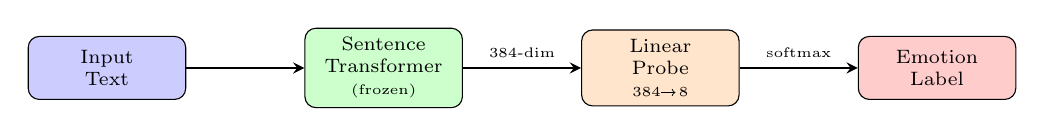
\begin{tikzpicture}[
    node distance=1.5cm,
    box/.style={rectangle, draw, rounded corners, minimum height=0.8cm, minimum width=2cm, align=center, font=\scriptsize},
    arrow/.style={->, thick, >=stealth}
]

\node[box, fill=blue!20] (input) {Input\\Text};
\node[box, fill=green!20, right=of input] (embed) {Sentence\\Transformer\\{\tiny (frozen)}};
\node[box, fill=orange!20, right=of embed] (probe) {Linear\\Probe\\{\tiny 384→8}};
\node[box, fill=red!20, right=of probe] (output) {Emotion\\Label};

\draw[arrow] (input) -- (embed);
\draw[arrow] (embed) -- node[above, font=\tiny] {384-dim} (probe);
\draw[arrow] (probe) -- node[above, font=\tiny] {softmax} (output);

\end{tikzpicture}
\end{center}

\vspace{0.3cm}

\begin{columns}[T]
\column{0.5\textwidth}
\textbf{Model:}
\begin{itemize}
    \item Pre-trained embedder (66M params frozen)
    \item 2-layer MLP (49K trainable)
    \item Fast inference (~100ms)
\end{itemize}

\column{0.5\textwidth}
\textbf{8 Emotion Classes:}
\begin{itemize}
    \item Calm, Confident, Defensive
    \item Dismissive, Passionate
    \item Frustrated, Angry, Sarcastic
\end{itemize}
\end{columns}
\end{frame}



\begin{frame}{Training Configuration}
\begin{columns}[T]

\column{0.5\textwidth}
\begin{block}{Hyperparameters}
\small
\begin{itemize}
    \item Adam optimizer, LR: 0.001
    \item Batch: 32, Epochs: 20
    \item Dropout: 0.3
    \item CrossEntropy loss
\end{itemize}
\end{block}

\column{0.5\textwidth}
\begin{block}{Why Linear Probe?}
\small
\begin{itemize}
    \item Only 49K trainable params
    \item Works with 400 examples
    \item Fast inference (~100ms)
    \item Low memory footprint
\end{itemize}
\end{block}

\end{columns}

\vspace{0.3cm}

\begin{center}
\textbf{Model:} 66M frozen + 49K trainable = 66M total params
\end{center}
\end{frame}

\begin{frame}{Testing Methodology}
\begin{block}{Test Setup}
\begin{itemize}
    \item GPT Generated 500 labeled examples using structured prompts for 8 emotion classes
    \item Split: 400 train / 100 val
    \item 100 held-out test (balanced)
\end{itemize}
\end{block}

\vspace{0.2cm}

\begin{block}{Evaluation Process}
\begin{enumerate}
    \item Train 20 epochs, validate, select best
    \item Test on 100 held-out examples
    \item Real-world validation on recordings
\end{enumerate}
\end{block}

\vspace{0.2cm}

\begin{alertblock}{Note}
Synthetic data provides strong baseline for transfer learning
\end{alertblock}
\end{frame}

\begin{frame}{Emotion Classifier Results}
\begin{table}
\centering
\small
\begin{tabular}{lccc}
\toprule
\textbf{Metric} & \textbf{Mean} & \textbf{Std} & \textbf{Range} \\
\midrule
Accuracy & \textbf{73.2\%} & 4.1\% & 68-79\% \\
Precision & 71.8\% & 5.2\% & 64-78\% \\
Recall & 72.4\% & 4.8\% & 66-78\% \\
F1-Score & 72.1\% & 4.5\% & 66-78\% \\
\bottomrule
\end{tabular}
\end{table}

\vspace{0.3cm}

\begin{columns}[T]
\column{0.5\textwidth}
\textbf{Best Classes:}
\begin{itemize}
    \item Angry: 82\% F1
    \item Confident: 79\% F1
    \item Calm: 76\% F1
\end{itemize}

\column{0.5\textwidth}
\textbf{Challenging:}
\begin{itemize}
    \item Sarcastic: 65\% F1
    \item Defensive: 68\% F1
\end{itemize}
\end{columns}

\vspace{0.2cm}

\begin{alertblock}{Insight}
73\% for 8-way classification with only 400 examples!
\end{alertblock}
\end{frame}

% ====================
% SECTION 4: RAG SYSTEM
% ====================
\section{Fact-Checking with RAG}

\begin{frame}{Multi-Source Fact-Checking Pipeline}
\begin{center}
\begin{tikzpicture}[
    node distance=0.7cm and 1.5cm,
    box/.style={rectangle, draw, rounded corners, minimum height=0.6cm, minimum width=1.8cm, align=center, font=\tiny},
    arrow/.style={->, thick, >=stealth}
]

% Input
\node[box, fill=blue!20] (query) {Query};

% Three parallel sources
\node[box, fill=green!20, below left=1cm and 0.8cm of query] (kb) {�� KB\\RAG};
\node[box, fill=purple!20, below=1cm of query] (poly) {�� Polymarket\\Cache};
\node[box, fill=orange!20, below right=1cm and 0.8cm of query] (web) {�� Web\\DDG};

% Combine
\node[box, fill=red!20, below=2cm of query] (combine) {Aggregate};

% Output
\node[box, fill=yellow!20, below=of combine] (output) {Facts};

% Arrows
\draw[arrow] (query) -- (kb);
\draw[arrow] (query) -- (poly);
\draw[arrow] (query) -- (web);
\draw[arrow] (kb) -- (combine);
\draw[arrow] (poly) -- (combine);
\draw[arrow] (web) -- (combine);
\draw[arrow] (combine) -- (output);

\end{tikzpicture}
\end{center}

\vspace{0.2cm}
\small
\textbf{Three Sources:} �� Curated KB (semantic) | �� Polymarket (crowd opinion) | �� Web (current news)
\end{frame}



\begin{frame}{RAG: Vector Database Architecture}
\begin{center}
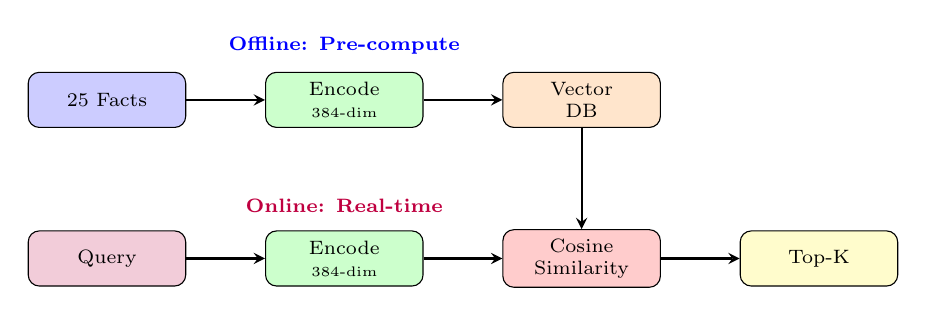
\begin{tikzpicture}[
    node distance=1cm,
    box/.style={rectangle, draw, rounded corners, minimum height=0.7cm, minimum width=2cm, align=center, font=\scriptsize},
    arrow/.style={->, thick, >=stealth}
]

% Offline indexing (top)
\node[box, fill=blue!20] (facts) {25 Facts};
\node[box, fill=green!20, right=of facts] (embed_offline) {Encode\\{\tiny 384-dim}};
\node[box, fill=orange!20, right=of embed_offline] (store) {Vector\\DB};
\draw[arrow] (facts) -- (embed_offline);
\draw[arrow] (embed_offline) -- (store);
\node[above=0.1cm of embed_offline, font=\scriptsize\bfseries\color{blue}] {Offline: Pre-compute};

% Online search (bottom)
\node[box, fill=purple!20, below=1.3cm of facts] (query) {Query};
\node[box, fill=green!20, right=of query] (embed_online) {Encode\\{\tiny 384-dim}};
\node[box, fill=red!20, right=of embed_online] (cosine) {Cosine\\Similarity};
\node[box, fill=yellow!20, right=of cosine] (topk) {Top-K};

\draw[arrow] (query) -- (embed_online);
\draw[arrow] (embed_online) -- (cosine);
\draw[arrow] (store.south) -- ++(0,-0.3) -| (cosine.north);
\draw[arrow] (cosine) -- (topk);
\node[above=0.1cm of embed_online, font=\scriptsize\bfseries\color{purple}] {Online: Real-time};

\end{tikzpicture}
\end{center}

\vspace{0.2cm}

\begin{itemize}
    \item \textbf{Model:} all-MiniLM-L6-v2, \textbf{Dimension:} 384
    \item \textbf{Metric:} Cosine similarity, \textbf{Threshold:} 0.3 (30\% match)
\end{itemize}
\end{frame}

\begin{frame}[fragile]{RAG: Knowledge Base Search}
\begin{block}{Semantic Search Algorithm}
\begin{lstlisting}[language=Python, basicstyle=\ttfamily\tiny, frame=single]
def search(query, top_k=3, threshold=0.3):
    # Encode query to 384-dim vector
    query_emb = model.encode(query)

    # Cosine similarity with all facts
    sims = cosine_similarity(query_emb, fact_embeddings)

    # Return top-k above threshold
    top_idx = argsort(sims)[-top_k:]
    return [facts[i] for i in top_idx if sims[i] >= threshold]
\end{lstlisting}
\end{block}

\vspace{0.2cm}
\textbf{Key Steps:} Encode query $\rightarrow$ Compute similarity $\rightarrow$ Filter by threshold $\rightarrow$ Return top matches
\end{frame}

\begin{frame}{Polymarket Integration with LRU Caching}
\begin{center}
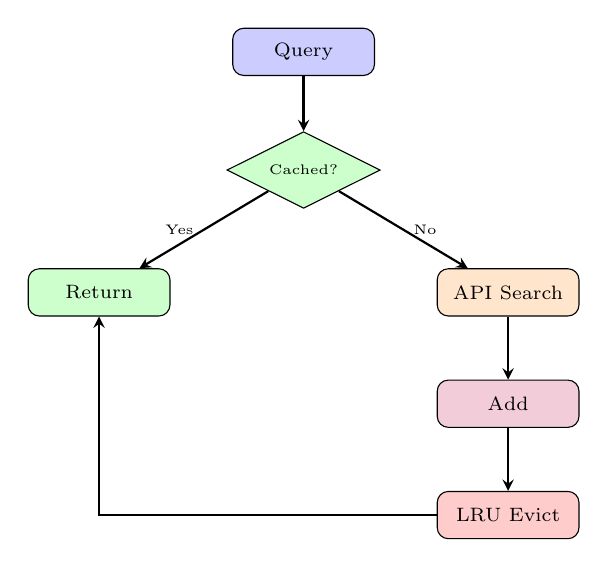
\begin{tikzpicture}[
    node distance=0.8cm,
    box/.style={rectangle, draw, rounded corners, minimum height=0.6cm, minimum width=1.8cm, align=center, font=\scriptsize},
    decision/.style={diamond, draw, fill=green!20, text width=1cm, align=center, aspect=2, font=\tiny},
    arrow/.style={->, thick, >=stealth}
]

\node[box, fill=blue!20] (query) {Query};
\node[decision, below=0.7cm of query] (cache) {Cached?};
\node[box, fill=green!20, below left=1cm and 1.2cm of cache] (return_cache) {Return};
\node[box, fill=orange!20, below right=1cm and 1.2cm of cache] (api) {API Search};
\node[box, fill=purple!20, below=of api] (add) {Add};
\node[box, fill=red!20, below=of add] (evict) {LRU Evict};

\draw[arrow] (query) -- (cache);
\draw[arrow] (cache) -- node[left, font=\tiny] {Yes} (return_cache);
\draw[arrow] (cache) -- node[right, font=\tiny] {No} (api);
\draw[arrow] (api) -- (add);
\draw[arrow] (add) -- (evict);
\draw[arrow] (evict) -| (return_cache);

\end{tikzpicture}
\end{center}


\end{frame}

\begin{frame}{Web Search Integration}
\begin{center}
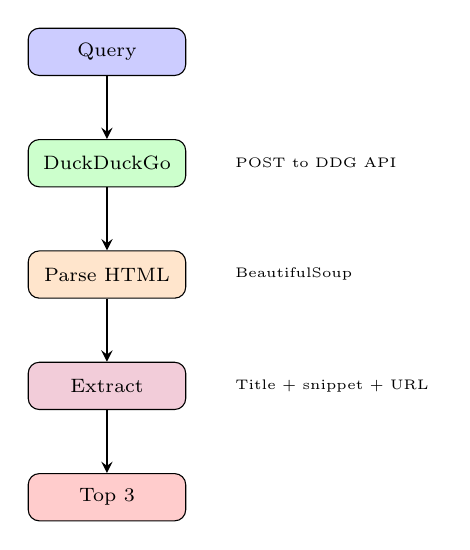
\begin{tikzpicture}[
    node distance=0.8cm,
    box/.style={rectangle, draw, rounded corners, minimum height=0.6cm, minimum width=2cm, align=center, font=\scriptsize},
    arrow/.style={->, thick, >=stealth}
]

\node[box, fill=blue!20] (query) {Query};
\node[box, fill=green!20, below=of query] (ddg) {DuckDuckGo};
\node[box, fill=orange!20, below=of ddg] (parse) {Parse HTML};
\node[box, fill=purple!20, below=of parse] (extract) {Extract};
\node[box, fill=red!20, below=of extract] (top3) {Top 3};

\draw[arrow] (query) -- (ddg);
\draw[arrow] (ddg) -- (parse);
\draw[arrow] (parse) -- (extract);
\draw[arrow] (extract) -- (top3);

% Compact annotations
\node[right=0.5cm of ddg, text width=2.5cm, font=\tiny] {POST to DDG API};
\node[right=0.5cm of parse, text width=2.5cm, font=\tiny] {BeautifulSoup};
\node[right=0.5cm of extract, text width=2.5cm, font=\tiny] {Title + snippet + URL};

\end{tikzpicture}
\end{center}

\vspace{0.2cm}

\begin{itemize}
    \item \textbf{Fallback} when KB/Polymarket lack info
    \item \textbf{Speed:} 1-2 sec, \textbf{Purpose:} Latest news
\end{itemize}
\end{frame}

% ====================
% SECTION 5: USE CASES
% ====================
\section{Use Cases}

\begin{frame}{Use Case 1: Corporate Decision-Making with Public Sentiment}
\begin{block}{Scenario}
Marketing team debating which F1 driver to approach for a brand partnership, based on public perception and championship momentum
\end{block}

\textbf{How System Helps:}
\begin{itemize}
    \item \textbf{Emotion Tracking:} Identifies when discussion becomes biased or emotionally charged
    \item \textbf{Fact-Checking:} Surfaces real-time public sentiment data from prediction markets
    \item \textbf{De-escalation:} Grounds debate in objective crowd-sourced probabilities
\end{itemize}

\vspace{0.3cm}

\begin{exampleblock}{Example: Max vs Lando F1 Championship Debate}
\textbf{Speaker A:} ``Max is the obvious choice -- everyone knows he'll win'' (Confident 82\%)\\
\textbf{Speaker B:} ``Lando has more momentum, the fans love him right now'' (Passionate 75\%)\\

\textbf{System shows:} Polymarket: Max 63\% vs Lando 28\% championship odds\\
Web: Recent fan sentiment analysis, social media engagement stats
\end{exampleblock}
\end{frame}

% ====================
% SECTION 6: RESULTS
% ====================
\section{Results \& Demo}

\begin{frame}{System Performance Metrics}
\begin{table}
\centering
\begin{tabular}{lcc}
\toprule
\textbf{Component} & \textbf{Metric} & \textbf{Value} \\
\midrule
\textbf{Raspberry Pi} & & \\
Speaker Diarization & Processing Time & 2-3 sec \\
Whisper Transcription & Processing Time & 2-3 sec \\
Total Pi Processing & Latency & 4-6 sec \\
\midrule
\textbf{AWS EC2} & & \\
Emotion Classifier & Accuracy & 73.2\% \\
Emotion Classifier & Inference Time & 100 ms \\
RAG Search & Query Time & 50 ms \\
Polymarket Lookup & Query Time & 80 ms \\
Web Search & Query Time & 1-2 sec \\
Total AWS Processing & Latency & 2-3 sec \\
\midrule
\textbf{End-to-End} & & \\
Total System Latency & Pi + AWS + Network & 6-10 sec \\
\bottomrule
\end{tabular}
\end{table}
\end{frame}



\begin{frame}{Live System Output}
\begin{center}
\includegraphics[width=0.9\textwidth,height=0.75\textheight,keepaspectratio]{s3.png}
\end{center}

\vspace{0.2cm}
\begin{center}
\small
live demo: http://54.209.249.85:7863/
\end{center}



\end{frame}

\begin{frame}{System Output Examples}
\begin{columns}[T]

\column{0.48\textwidth}
\begin{center}
\textbf{Chat Conversation View}
\includegraphics[width=\textwidth,height=0.6\textheight,keepaspectratio]{s1.png}
\end{center}
\small Speaker segments with emotion labels

\column{0.48\textwidth}
\begin{center}
\textbf{Analysis Panel}
\includegraphics[width=\textwidth,height=0.6\textheight,keepaspectratio]{s2.png}
\end{center}
\small Emotion metrics + Polymarket predictions

\end{columns}
\end{frame}

% ====================
% SECTION 7: FUTURE WORK
% ====================
\section{Future Directions}





% ====================
% CONCLUSION
% ====================
\section{Conclusion}

\begin{frame}{Summary}
\begin{block}{What We Built}
A distributed edge-cloud system for real-time conversation analysis:
\begin{itemize}
    \item \textbf{73.2\%} emotion accuracy (8 classes)
    \item \textbf{3-source} fact-checking: RAG + Polymarket + Web
    \item \textbf{6-10 sec} end-to-end latency
\end{itemize}
\end{block}

\vspace{0.2cm}

\begin{block}{Key Innovations}
\begin{enumerate}
    \item Hybrid fact-checking with prediction markets
    \item LRU-cached market discovery
    \item Segment-level emotion analysis
    \item Privacy-preserving edge architecture
\end{enumerate}
\end{block}

\vspace{0.2cm}

\begin{alertblock}{Impact}
Reduces bias by providing objective facts and public opinion data
\end{alertblock}
\end{frame}

\begin{frame}{Thank You}
\begin{center}
\Huge Thank You!

\vspace{1cm}

\Large Questions?

\vspace{1cm}

\normalsize
\textbf{Project Links:}\\
\vspace{0.3cm}
GitHub: \texttt{github.com/ifesionubogu/aiot\_project}\\
Live Demo: \texttt{http://54.209.249.85:7863/}\\
Technical Report: See \texttt{TECHNICAL\_REPORT.pdf}

\end{center}
\end{frame}

\end{document}
